\section{Results}
\label{results}

We divided the evaluation into two phases. In the first one, we examined the process of learning each strategy and the results. For the second one, we tested their performance during gameplay. The presented results ran on a 2.6 GHz Quad-Core Intel Core i7 processor under MacOs. The benchmarks were performed using three different initial configurations for each game of increasing complexity, namely, \textit{Small(S), Medium(M)} and \textit{Large(L)}. These divisions were designed to provide information about the scalability of each approach into the \textit{Classical} initial setting.

\newcommand\nimcirc[3]{ 
    \filldraw[fill=black!7] (#1+#2*0.8,#3*0.8) circle (0.2cm) node {};
}
\newcommand\nimcircg[3]{ 
    \filldraw[fill=green!7] (#1+#2*0.8,#3*0.8) circle (0.2cm) node {};
}
\begin{figure}[H]
    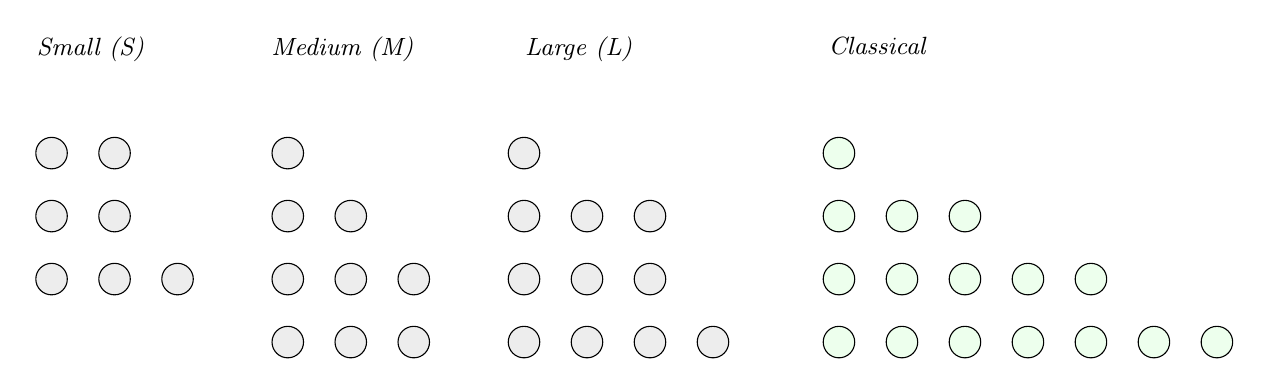
\begin{tikzpicture}
    \nimcirc{0}{0}{1}
    \nimcirc{0}{1}{1}
    \nimcirc{0}{2}{1}

    \nimcirc{0}{0}{2}
    \nimcirc{0}{1}{2}

    \nimcirc{0}{0}{3}
    \nimcirc{0}{1}{3}

    \node[below, font=\small] at (0.5,4) {\textit{Small (S)}};

    \nimcirc{3}{0}{0}
    \nimcirc{3}{1}{0}
    \nimcirc{3}{2}{0}

    \nimcirc{3}{0}{1}
    \nimcirc{3}{1}{1}
    \nimcirc{3}{2}{1}

    \nimcirc{3}{0}{2}
    \nimcirc{3}{1}{2}

    \nimcirc{3}{0}{3}

    \node[below, font=\small] at (3.7,4) {\textit{Medium (M)}};

    \nimcirc{6}{0}{0}
    \nimcirc{6}{1}{0}
    \nimcirc{6}{2}{0}
    \nimcirc{6}{3}{0}

    \nimcirc{6}{0}{1}
    \nimcirc{6}{1}{1}
    \nimcirc{6}{2}{1}

    \nimcirc{6}{0}{2}
    \nimcirc{6}{1}{2}
    \nimcirc{6}{2}{2}

    \nimcirc{6}{0}{3}

    \node[below, font=\small] at (6.7,4) {\textit{Large (L)}};

    \nimcircg{10}{0}{0}
    \nimcircg{10}{1}{0}
    \nimcircg{10}{2}{0}
    \nimcircg{10}{3}{0}
    \nimcircg{10}{4}{0}
    \nimcircg{10}{5}{0}
    \nimcircg{10}{6}{0}

    \nimcircg{10}{0}{1}
    \nimcircg{10}{1}{1}
    \nimcircg{10}{2}{1}
    \nimcircg{10}{3}{1}
    \nimcircg{10}{4}{1}

    \nimcircg{10}{0}{2}
    \nimcircg{10}{1}{2}
    \nimcircg{10}{2}{2}

    \nimcircg{10}{0}{3}

    \node[below, font=\small] at (10.5,4) {\textit{Classical}};

    \end{tikzpicture}
    \caption{Initial configurations for \textit{Nim}.} 
\end{figure}

\begin{figure}[H]
        \begin{tikzpicture}[scale=0.95]
    \newcommand\x{0}
    \draw[step=0.7cm,draw=black!60,very thin,
    fill=black!7] (\x+0,0) grid (\x+2.1,2.1) rectangle (\x+0,0);
    \draw[thick] (\x+1.05,1.75) node{a};
    \draw[thick] (\x+1.75,0.35) node{b};
    \draw[thick] (\x+0.35,1.75) node{b};
    
    \node[below, font=\small] at (1,3) {\textit{Small (S)}};

    \newcommand\xx{3.5}
    \draw[step=0.7cm,draw=black!60,very thin,
    fill=black!7] (\xx+0,0) grid (\xx+2.1,2.1) rectangle (\xx+0,0);
    \draw[thick] (\xx+0.35,0.35) node{a};
    \draw[thick] (\xx+1.75,0.35) node{b};
    \node[below, font=\small] at (4.5,3) {\textit{Medium (M)}};
    
    
    \newcommand\xxx{7}
    \draw[step=0.7cm,draw=black!60,very thin,
    fill=black!7] (\xxx+0,0) grid (\xxx+2.1,2.1) rectangle (\xxx+0,0);
    \draw[thick] (\xxx+1.75,1.75) node{a};
    
    \node[below, font=\small] at (7.7,3) {\textit{Large (L)}};
    
    \newcommand\xxxx{11.2}
    \draw[step=0.7cm,draw=black!60,very thin,
    fill=green!07] (\xxxx+0,0) grid (\xxxx+2.1,2.1) rectangle (\xxxx+0,0);
    
    \node[below, font=\small] at (11.8,3) {\textit{Classical}};
    
    
\end{tikzpicture}
\caption{Initial configurations for \textit{TicTacToe}} 
    \label{nim_sample}
    \end{figure}


\subsection{Learning phase}

The learning phase of the evaluation consisted of computing the strategy for each approach. The strategies were computed for each initial state and saved for the next phase. We will proceed to interpret different aspects of the this process as well as the resulted strategies. 

\begin{minipage}{0.5\linewidth}
    \centering
    \begin{table}[H]
        \small
        \setlength{\tabcolsep}{0.5em}
        \def\arraystretch{1.1}
        \begin{threeparttable}
            \begin{tabular}{L{0.30\linewidth} p{0.09\linewidth}p{0.09\linewidth}p{0.1\linewidth}}
                \toprule[0.25mm]
                Approach & S & M & L
                \\
                \midrule[0.35mm]
                Minimax  & 390 & 4630 & 61023
                \\[20pt]
                Pruned minimax tree   & 83 & 347 & 2675
                \\[20pt]
                Pruned minimax rules & 35 & 85 & 283 
                \\
                \bottomrule[0.25mm]
            \end{tabular}
            \caption{Number of nodes in the computed tree for Nim}
        \end{threeparttable}
    \end{table}
\end{minipage}
\begin{minipage}{0.5\linewidth}
    \centering
    \begin{table}[H]
        \small
        \setlength{\tabcolsep}{0.5em}
        \def\arraystretch{1.1}
        \begin{threeparttable}
            \begin{tabular}{L{0.30\linewidth} p{0.09\linewidth}p{0.09\linewidth}p{0.1\linewidth}}
                \toprule[0.25mm]
                Approach & S & M & L
                \\
                \midrule[0.35mm]
                Minimax  & 896 & 7583 & 59704
                \\[20pt]
                Pruned minimax tree   & 105 & 73 & 2835
                \\[20pt]
                Pruned minimax rules & 109 & 61 & 2399 
                \\
                \bottomrule[0.25mm]
            \end{tabular}
            \caption{Number of nodes in the computed tree for TicTacToe}
        \end{threeparttable}
    \end{table}
\end{minipage}

The trees computed for the Minimax and the Pruned Minimax approaches are too large to be presented in this paper. Nevertheless, we can examine their structure by looking at the number of nodes in each tree. Such numbers are included in Figure 16 and their detailed values can be found in Tables 1 and 2. From those tables, we can notice the significant reduction in the tree size when using the pruning strategy compared to the full tree. As well as a further reduction by including the learned rules in the learning.

Unlike game trees, the weak constraints generated by the ILASP approach for each initial instance are concise and explainable. The strategy found for Nim (Figure 16), encode the mathematical strategy explained along with the game description. Lines 1, 2 and 3 define new predicates \texttt{nim\_sum/3} and \texttt{b/3} to save the \textit{Nim Sum} and the binary number of each digit for every pile, respectively. Using this new predicates, the weak constraint in line 4 penalizes an odd \textit{Nim Sum} for any digit. The strategy learned using the small instance only varies by penalizing \textit{nim\_sum(V0,V1,3)} instead of \textit{nim\_sum(V0,V1,4)}, this change is associated to the lack of counters on pile 4 for the small instance. 

The strategy found for TicTacToe with initial state \textit{M} (Figure 18) will give preference to stable models where there is a free space in a consecutive line, stated in line 1. A higher priority of 2 will be assigned to stable models where player $V0$, corresponding to the current player, completes a full line in the next state. This last fact encoded in lines 2 and 3, corresponds to the expected strategy of always choosing the action leading to a winning state. In the case of the initial state \textit{S} (Figure 17), lines 3 and 4 will penalize actions where the next state has a line with one cell taken and one free. Thus, encouraging actions that block the other player moves.  

\begin{center}
    \begin{lstlisting}[] 
nim_sum(V1,0,0) :- b(_,V1,_).
nim_sum(V1,V3+V2,V0) :- b(V0,V1,V2), nim_sum(V1,V3,V0-1).
b(V3,V1,V2) :- binary(V0,V1,V2), next(has(V3,V0)).
:~ nim_sum(V0,V1,4), V1\2 != 0.[1@1, 4, V0, V1]
    \end{lstlisting}
    \captionof{figure}{Strategy found by ILASP for Nim instances \textit{M} and \textit{L}}
\end{center}

\begin{center}
    \begin{lstlisting}[] 
:~ next(has(V0,V1)), in_line(V1,V2,V3).[1@1, 1, V0, V1, V2, V3]
:~ in_line(V0,V1,V2), next(free(V0)).[-1@2, 2, V0, V1, V2]
:~ next(has(V0,V1)), in_line(V2,V3,V1), 
   next(free(V2)).[1@2, 3, V0, V1, V2, V3]
:~ next(has(V0,V1)), next(has(V0,V2)), 
   next(has(V0,V3)), in_line(V1,V2,V3).[-1@2, 4, V0, V1, V2, V3]
    \end{lstlisting}
    \captionof{figure}{Strategy found by ILASP for TicTacToe instance \textit{S}}
\end{center}

\begin{center}
    \begin{lstlisting}[] 
:~ in_line(V0,V1,V2), next(free(V2)).[-1@1, 1, V0, V1, V2]
:~ next(has(V0,V1)), next(has(V0,V2)), 
   next(has(V0,V3)), in_line(V1,V2,V3).[-1@2, 2, V0, V1, V2, V3]
    \end{lstlisting}
    \captionof{figure}{Strategy found by ILASP for TicTacToe instance \textit{M}}
\end{center}



We present in Figure 16 the time taken by each approach to generate the strategy. These times are taking into account the saving process for each strategy, in the case of strategies in the form of trees, this process exported the tree into JSON format to provide faster access. The building times for ILASP include the generation of ordered examples from the Pruned Minimax approach as well as the ILASP process to compute the Hypothesis.

We notice how for the small TicTacToe the times for ILASP are considerably bigger than the rest. This overload is due to the abstraction process of ILASP, while the rest of the approaches can quickly compute a strategy for a small instance. For the medium size, we can notice that the Minimax approach takes the most time while Pruned Minimax learning rules takes the least time. This behavior correlates with the number of explored nodes. For the larger instance, there are some key points to notice. First, we can see how the game of Nim behaves as it does for the medium size with Pruned Minimax, whereas for TicTacToe we can see a drastic change. In the case of ILASP no strategy was found to cover all the ordered examples. 
% The examples that provoked it were those referring to earlier stages of the game where a clear strategy is hard to find even for a human. Such cases must see over 2 steps into the future to make the decision. 
Pruned Minimax with rules outperformed the rest of the approaches in almost every configuration, while for the large TicTacToe instance we can see a bad performance.
% We can attribute this increase in time to the lack of abstraction used for the game. The rules generated for this game consist of only constants and only abstract players, unlike the ones presented for Nim where the pile numbers are substituted by variables. As a result, the number of rules for the strategy increases, generating over 1000 rules that are included in each call to \textit{clingo} slowing down its response. 

\begin{figure}[H]
    \centering
    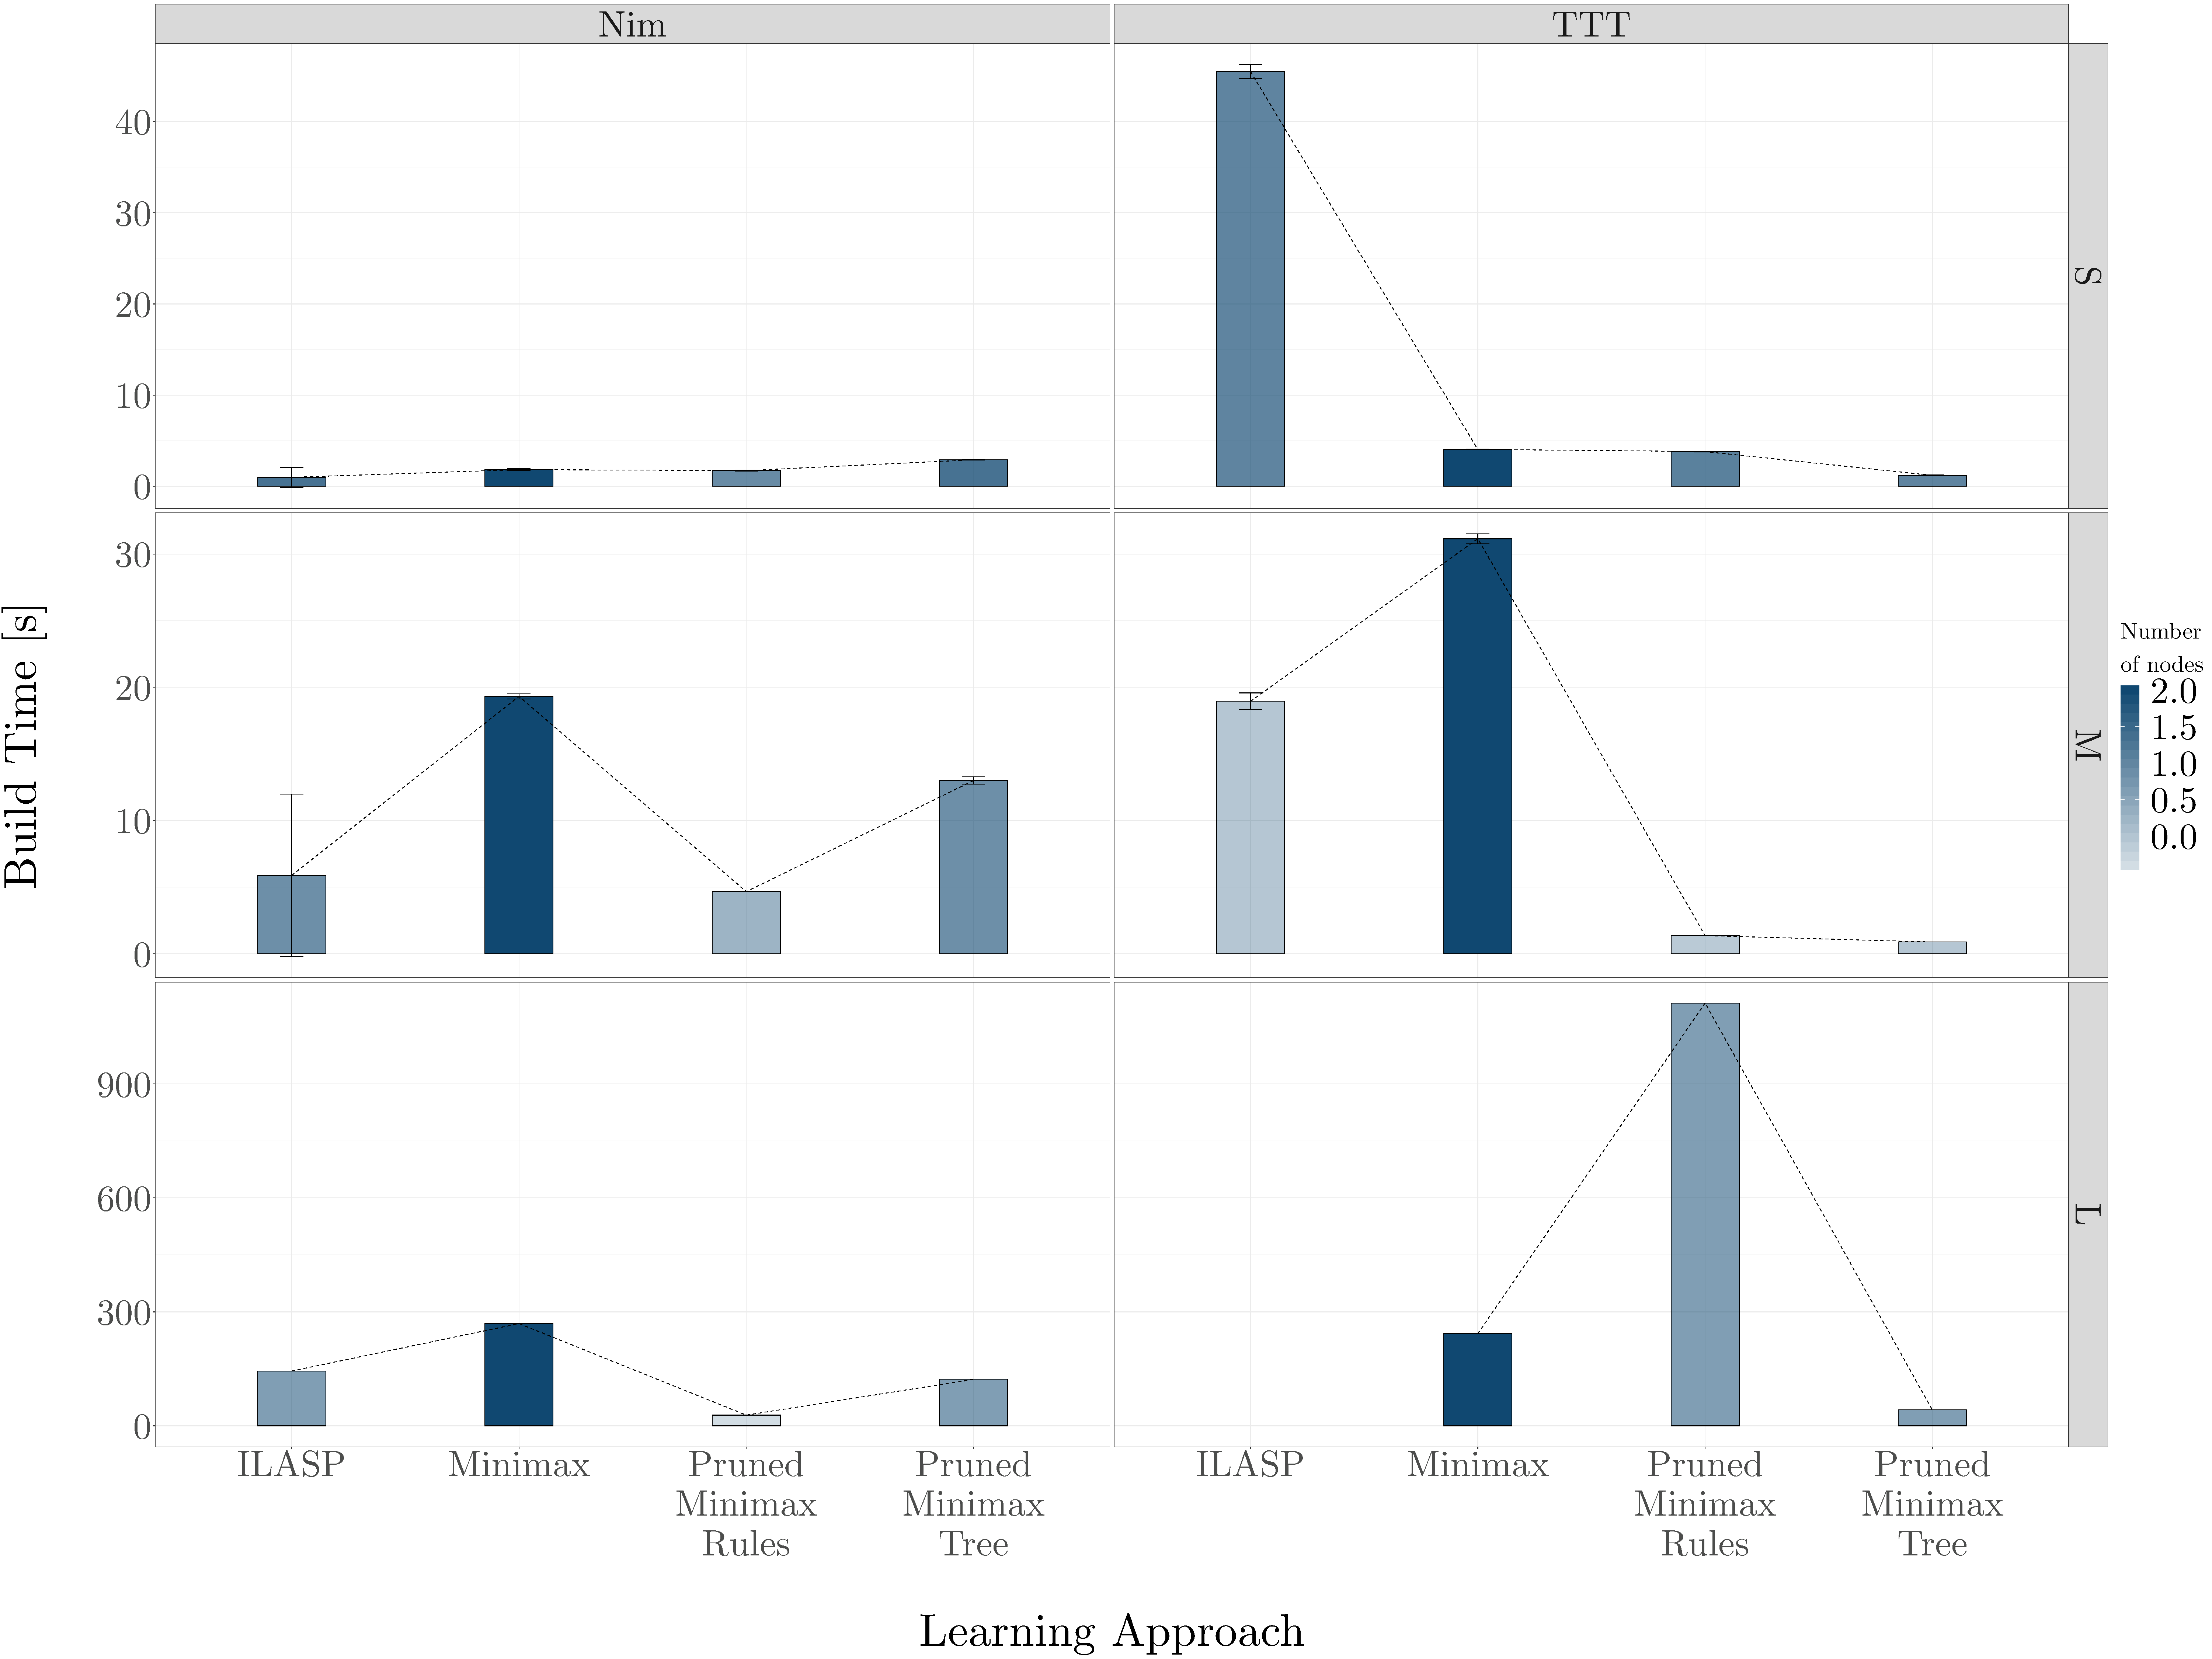
\includegraphics[width=\linewidth]{bar_build.pdf}
    \caption{Learning times for each approach. The bar colors are computed applying $log_{10}$ to the proportion of nodes, with 100 being the tree with the most nodes for each game and size.}
\end{figure}

\subsection{Approaches against Random-Agent}

For each learning approach, we created an agent with the capability to choose an action in the current state of the game $s_c$. This judgment is based on the generated strategies during the learning phase. Table 3 gives a summary of how each agent will select an action during gameplay. 

\begin{table}[H]
	\centering
	\small
	\setlength{\tabcolsep}{0.5em}
	\def\arraystretch{1.1}
	\begin{threeparttable}
		\begin{tabular}{L{0.15\linewidth} p{0.25\linewidth} p{0.5\linewidth}}
			\toprule[0.25mm]
            Agent & Strategy & Action selection for current state $s_c$ 
            \\
			\midrule[0.35mm]
            Minimax  & Full minimax tree 
            &Finds a node in the tree with for state $s_c$ and choose the action corresponding to the children which maximizes the score. If no node is found for $s_c$, choose a random action.
            \\[20pt]
            Pruned minimax tree   & Pruned minimax tree 
            & Same as Minimax agent. The unexplored sections of the tree will increase the likelihood of $s_c$ not being part of the tree.
            \\[20pt]
            Pruned minimax rules & ASP rules   
            & Includes the rules as part of the clingo call and selects one of the remaining stable models. 
            \\[20pt]
            ILASP & Weak constraints  
            & Includes the weak constrains as part of the clingo call and selects the optimal stable model.
            \\
			\bottomrule[0.25mm]
		\end{tabular}
		\caption{Tabular summary of learned strategies}
	\end{threeparttable}
\end{table}

\begin{figure}[H]
    \centering
    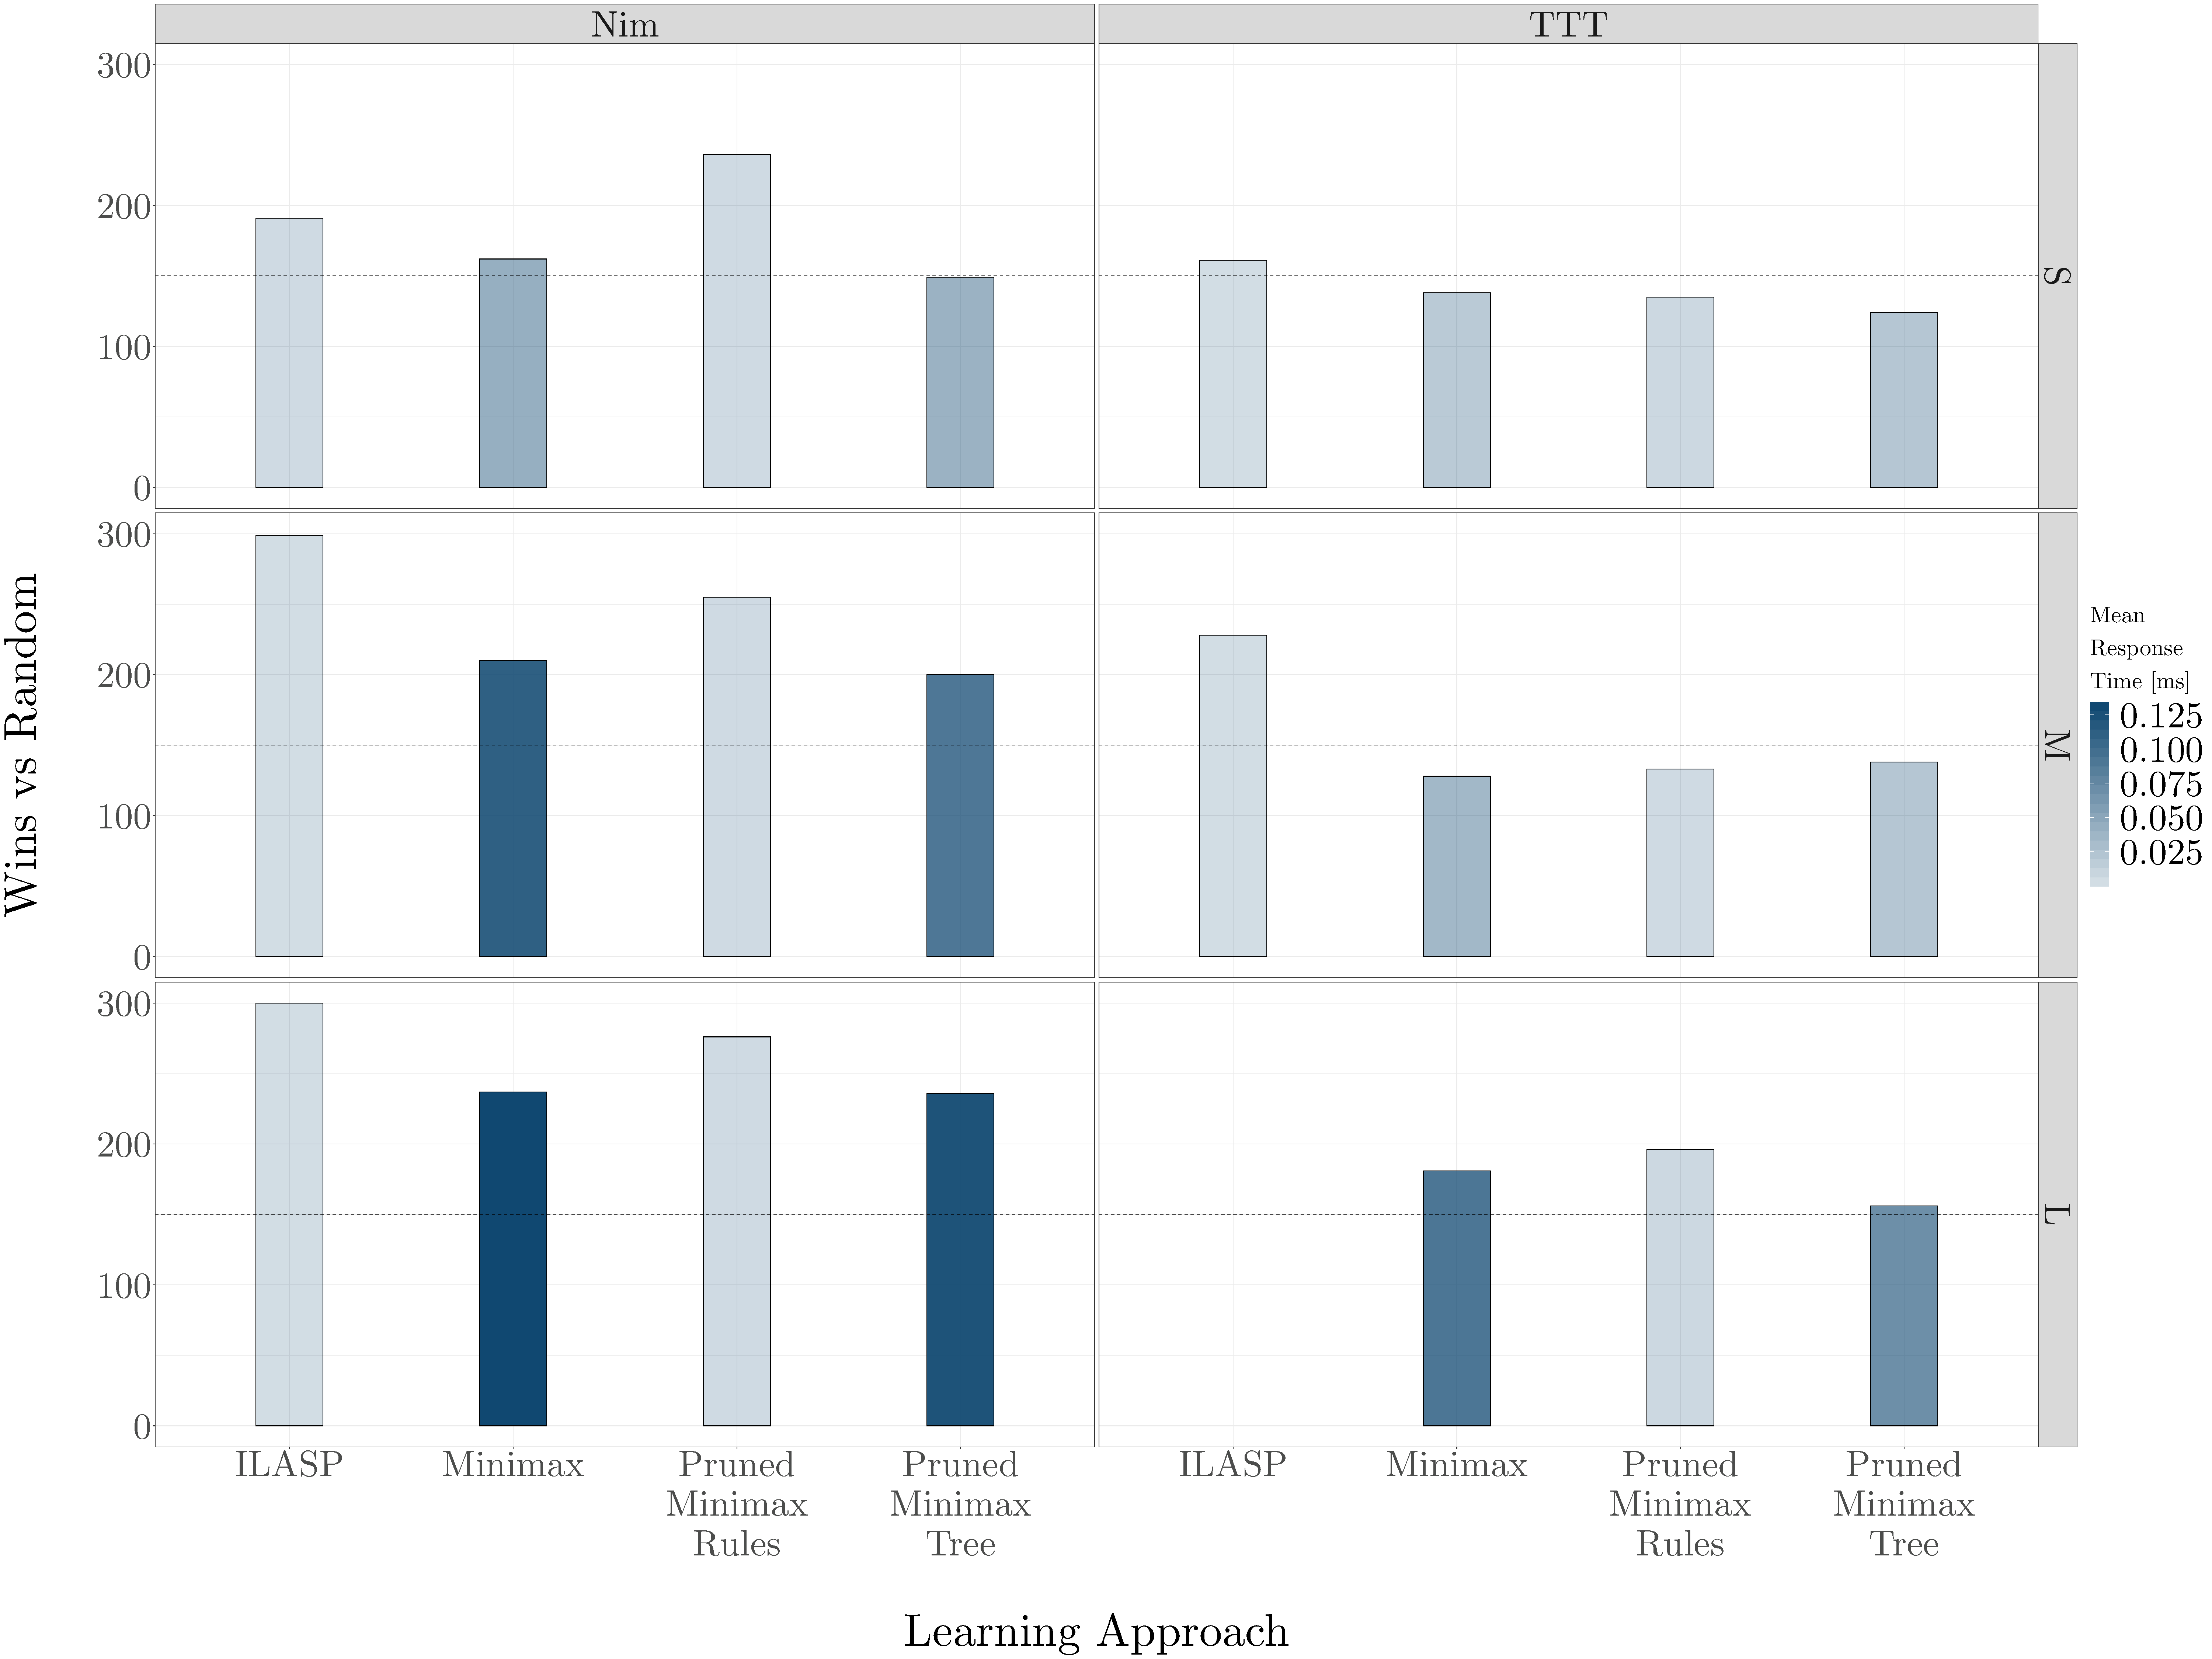
\includegraphics[width=\linewidth]{bar_vs.pdf}
    \caption{Number of winning matches for each approach against a random agent including their mean response time.}
\end{figure}

We played each agent against a Random-Agent and compared the number of wined matches in Figure 20. Using the classical initial state, we simulated a total of 300 matches switching the starting player in each game to avoid an initial advantage to either player. 

We can see that out of all approaches that learned from small instances, only the ILASP strategy was able to outperform the random agent in TicTacToe. This behavior continued throughout the experiment showing the potential of ILASP to generalize into bigger instances. For the game of Nim, the Pruned Minimax agent working with rules was also able to generalize and wan against the random agent in over 75\% of the matches. We can also notice a slight improvement when using the full Minimax tree instead of the pruned tree in both games. Regarding the response times, it is easy to notice the increment on response times for indexing the tree. While, on the other hand, adding more information to the encoding showed to provide a fast response.

\subsection{Framework}

In addition to the research performed on these approaches, we made available a generalized framework. With this framework, we want to encourage the use and research of ASP in two-player games. Our implementation allows simple expansions for new games following the GLD formalisms as well as new approaches for learning strategies. These expansions will automatically generate the command-line tools to build strategies, create agents and compute benchmarks. We also make available the tree visualizations by simply defining an ASCII representation of the states for the new game. The code can be found in \href{https://github.com/atreyasha/asp-game-strategies}{github}\footnote{https://github.com/susuhahnml/asp-game-strategies}, including a detailed explanation of how to extend it with new games and approaches. 



\section{Discussion}
\label{discussion}

A deeper analysis of the results showed different issues and advantages in each approach taken. Computing the full Minimax tree showed to be generally inefficient. We can see an expected exponential blowup in the number of nodes that correlates with the computation and response times. This outcome was expected as it is related to the brute-force nature of the algorithm. By pruning the tree we notice a clear improvement in the number of nodes. This improvement will also depend on the specific instance and the ordered in with actions are explored. It was due to this random factor that the algorithm was able to skip a big part of the tree in the medium TicTacToe instance, leading to fewer nodes than the ones from the small instance. Even though the pruning had better overall run times and improved space, the contrasting outcome can be seen in the slight difference in performance during gameplay. We can attribute this decrease on winned games, compared to plain Minimax, to the cases where the gameplay falls into the unexplored states of the pruned tree resulting in a random action instead of an informed one.

By learning ASP rules that abstracted the Pruned Minimax tree, we can notice an improvement in the scalability and the number of nodes. This improvement, however, was not the same for both games. By analyzing Figure 20 we can notice a very good performance for Nim, but a poor one for TicTacToe. This can be attributed to the level of abstraction in the rules generated for each game. In TicTacToe strategy rules consist of only constants except for the player's names, whereas the ones presented for Nim, the pile numbers are also substituted by variables. This result can also be seen in the increased build time for the larger instance of TicTacToe. In this case, the number of rules for the strategy increases, generating over 1000 rules that are included in each call to \textit{clingo} slowing down its response. 


Learning weak constraints with ILASP successfully generalized from small instances into the real game. However, it was not able to reach a conclusive strategy for the large instance of TicTacToe. We noticed that examples provoking this outcome were those referring to earlier stages of the game where a clear strategy is hard to find even for a human; such cases must see over 3 steps into the future to make the decision. The advantage that ILASP provided with explainable and simple strategies can arguably be outweighed by the complexity of the language bias. While the language bias for TicTacToe was intuitive, the one for Nim had to be carefully handcrafted based on previous knowledge of the expected strategy. 
